\documentclass[11pt]{article}
\usepackage[margin=1.5cm]{geometry}
\usepackage{amsmath,amssymb}
\usepackage{enumitem}
\usepackage{tikz}
\usepackage{listings}
\usepackage[T1]{fontenc}
\setlength{\columnsep}{0.7cm}
\setlength{\parindent}{0pt}
\setlist{nosep,leftmargin=*}
\lstset{
  basicstyle=\ttfamily\scriptsize,
  columns=fullflexible,
  keepspaces=true,
  aboveskip=2pt,
  belowskip=2pt,
  frame=single,
  breaklines=true
}

\begin{document}
\twocolumn

\title{Chapter 13 Warm-Up: A 2D Vector Class}
\author{Prof. Jordan C. Hanson}
\date{\today}
\maketitle

\section{What Is a Vector?}

A 2D vector has an \(x\)-component and a \(y\)-component:
\[
\vec{v} = \langle x, y \rangle .
\]
Geometrically, we can think of it as an arrow from the origin to the
point \((x,y)\).

\begin{center}
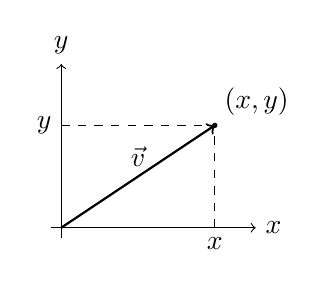
\begin{tikzpicture}[scale=0.65]
    \draw[->] (-0.2,0) -- (3.8,0) node[right] {\(x\)};
    \draw[->] (0,-0.2) -- (0,3.2) node[above] {\(y\)};
    \draw[->, thick] (0,0) -- (3,2) node[midway, above] {\(\vec{v}\)};
    \draw[dashed] (3,0) -- (3,2);
    \draw[dashed] (0,2) -- (3,2);
    \fill (3,2) circle (1.5pt);
    \node[below] at (3,0) {\(x\)};
    \node[left] at (0,2) {\(y\)};
    \node[above right] at (3,2) {\((x,y)\)};
\end{tikzpicture}
\end{center}

\section{Magnitude and Angle}

The \textbf{magnitude} of a vector is its length:
\[
|\vec{v}| = \sqrt{x^2 + y^2}.
\]

The \textbf{angle} \(\theta\) it makes with the positive \(x\)-axis is
\[
\theta = \tan^{-1}\left(\frac{y}{x}\right).
\]

\section{Build the Class and Add \\ Methods}

We can represent a vector using a class:

\begin{verbatim}
class Vector2D:
    def __init__(self, x, y):
        self.x = x
        self.y = y
\end{verbatim}

Begin your file with
\begin{verbatim}
import math
\end{verbatim}

Then add a magnitude method:

\begin{verbatim}
def magnitude(self):
    return math.sqrt(self.x**2+self.y**2)
\end{verbatim}

Add an angle method:

\begin{verbatim}
def angle(self):
    return math.atan2(self.y,self.x)
\end{verbatim}

What should
\begin{verbatim}
v1.magnitude()
\end{verbatim}
return for \(\langle 3,4\rangle\)?
\underline{\hspace{1.3cm}}

\section{Add and Subtract Vectors}

For
\[
\vec{u}=\langle x_1,y_1\rangle,
\qquad
\vec{v}=\langle x_2,y_2\rangle,
\]
vector addition is
\[
\vec{u}+\vec{v}
=
\langle x_1+x_2,\; y_1+y_2\rangle
\]
and subtraction is
\[
\vec{u}-\vec{v}
=
\langle x_1-x_2,\; y_1-y_2\rangle.
\]

Add these methods:

\begin{verbatim}
def __add__(self, other):
    return Vector2D(
        self.x+other.x,self.y+other.y)
def __sub__(self, other):
    return Vector2D(
        self.x-other.x,self.y-other.y)
\end{verbatim}

Test your addition and subtraction methods with
\begin{verbatim}
v1 = Vector2D(3, 4)
v2 = Vector2D(1, -2)
\end{verbatim}

\section{Looking Ahead: Inheritance}

A complex number $z = a + jb$ also has two components, much like a 2D vector.  How might you create a class
\texttt{ComplexNumber} that \textbf{inherits} from \texttt{Vector2D}?  What parts could it reuse? What new methods or meanings would it need? \textbf{Hint:} A child class can begin like this:
\begin{verbatim}
class ComplexNumber(Vector2D):
    ...
\end{verbatim}

\end{document}
